\section{Motivation}

A liquid-fueled \gls{MSR} is an advanced nuclear reactor with fissile material
dissolved in a molten salt mixture. This fuel salt mixture doubles as the primary reactor coolant
for transferring heat from the reactor core to the primary heat exchangers. Figure \ref{fig:msr}
shows a schematic diagram of a thermal-spectrum, channel-type \gls{MSR}. In channel-type
\glspl{MSR}, the fuel salt flows through vertical channels in the reactor core alongside neutron
moderators (e.g., graphite, heavy water, or molten sodium hydroxide). 
%
\begin{figure}[htb!]
	\centering
	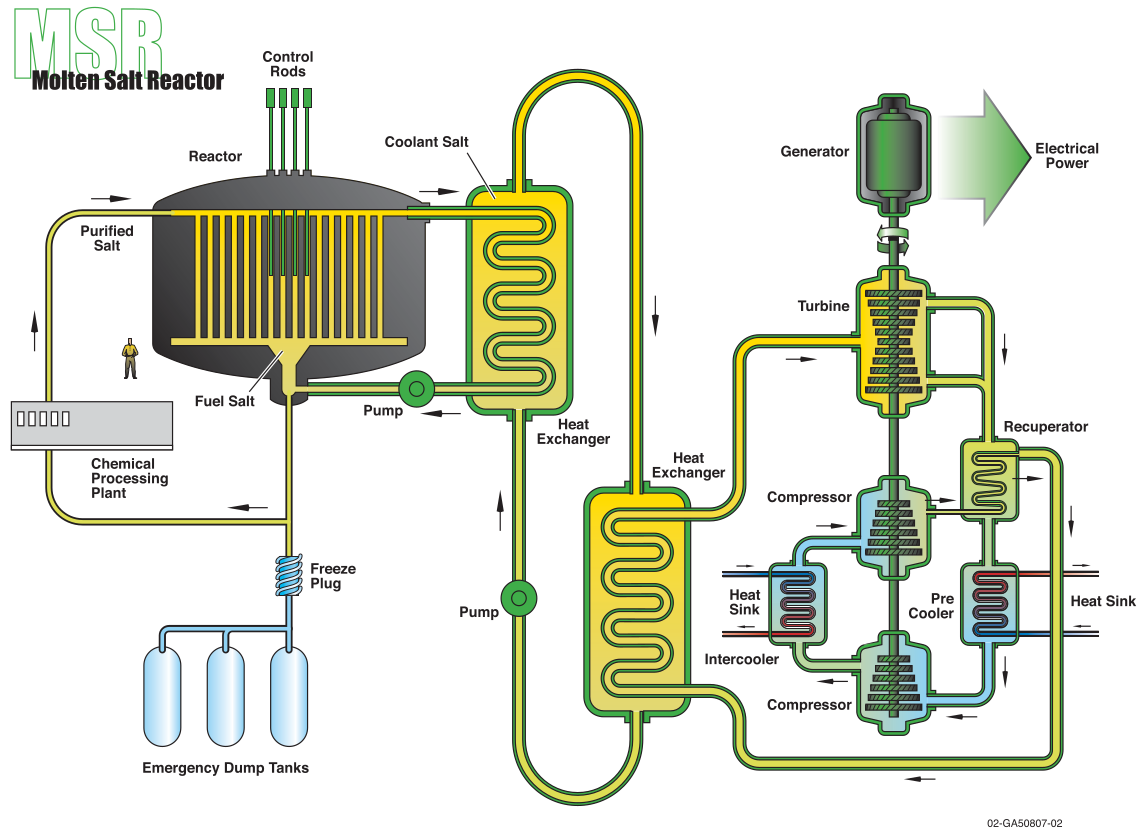
\includegraphics[width=.7\columnwidth]{msr}
	\caption{Schematic diagram of the \gls{MSR} concept. Retrieved from
	\cite{u.s._doe_nuclear_energy_research_advisory_committee_technology_2002}.}
	\label{fig:msr}
\end{figure}

The \gls{MSR} is one of six advanced reactor designs selected for improved safety, sustainability,
efficiency, and cost over the current generation of predominantly \glspl{LWR} at the \gls{GIF}.
Due to the high thermal expansion coefficient, \glspl{MSR} possess an inherently robust
safety feature in the strong negative fuel temperature coefficient of
reactivity \cite{elsheikh_safety_2013}. This reactivity coefficient limits the
maximum temperature that the reactor core would experience in an accident
scenario such as an unprotected reactivity insertion because the subsequent
rise in core temperatures induces a significant drop in reactivity,
quickly neutralizing the initial reactivity insertion. \glspl{MSR} also
operate at a large thermal margin to boiling and can rely on natural
circulation in the event of a pump failure. As a last resort, many \gls{MSR}
designs incorporate a drain plug made of actively-cooled frozen salt, which
melts when the core temperatures exceed safety thresholds. The hot molten salt
in the core would then flow into a drain tank designed to hold the fuel salt in
a subcritical configuration to disrupt any further chain fission reactions.

Some \glspl{MSR}, like the \gls{MSBR} or the \gls{MSFR}, can
incorporate the thorium fuel cycle for improved sustainability arising from the
use of abundant natural thorium resources and reduced transuranic waste
\cite{heuer_towards_2014}. The latter consequence also reduces costs
associated with long-term nuclear waste storage. Online fuel reprocessing raises the capacity
factor by reducing reactor downtime during reactor operation \cite{dolan_1_2017}.
Molten salt coolant loops can operate at near atmospheric pressures which eliminates the need for a
thick pressure vessel and drives down construction costs. We can make further economic arguments
supporting \glspl{MSR} in the context of the
carbon-constrained future envisioned in the \gls{IEA}'s \gls{NZE} roadmap
\cite{iea_net_2021}. The roadmap for minimizing carbon emissions requires solar photovoltaic- and
wind-dominated energy markets, which can results in highly variable and non-dispatchable
electricity generation. The resulting volatility in electricity prices
encourages the construction of heat storage and peak power
production plants. At the same time, demand for carbon-neutral
fuel will rise as electrification is economically unfeasible
for some industries, such as the aviation and marine sectors, which depend on
energy-dense fuels for propulsion. As described by Forsberg
\cite{forsberg_market_2020}, the most cost-efficient options for heat storage, peak power
production, and carbon-neutral fuel production all require high-temperature heat.
This requirement favors \glspl{MSR} which can deliver heat at higher average
temperatures than \glspl{LWR} and \glspl{SFR}.

Significant hurdles still stand in the way of commercial \gls{MSR} deployment \cite{dolan_27_2017}.
Major technological challenges include the need for further research on \gls{MSR} safety analysis,
irradiation and corrosion behavior of \gls{MSR} structural components, fission product tracking
and processing, \gls{MSR} nuclear safeguards measures, and the development of \gls{MSR} hydraulic
and heat exchanger components.

\subsection{Past \& Present \gls{MSR} Research \& Development}

\gls{ORNL} researchers first conceived the \gls{MSR} concept in pursuit of a high-temperature
liquid fuel reactor for the US Aircraft Nuclear Propulsion program in
the 1950s \cite{rosenthal_molten-salt_1970}. They
built the first ever operational \gls{MSR}, the 2.5 MW$_{\text{th}}$
\gls{ARE} reactor at \gls{ORNL}. The successful demonstration of the \gls{ARE} spurred further
research into adapting \glspl{MSR} for civilian power generation \cite{rosenthal_molten-salt_1970}.
Continued \gls{MSR} research efforts culminated in designing constructing, and successfully
operating of the 8-MW$_{\text{th}}$, thermal-spectrum \gls{MSRE} with
graphite channels and a LiF-BeF$_2$-ZrF$_4$-UF$_4$ fuel salt mixture
\cite{haubenreich_experience_1970}. In addition to other operational achievements, the
\gls{MSRE} became the first reactor to run on $^{233}$U fuel bred from $^{232}$Th. Building on
their experience with the \gls{MSRE}, \gls{ORNL} proposed a new program for constructing and
operating a demonstration reactor based on the \gls{MSBR} concept, which they had also developed
\cite{macpherson_molten_1985}. The \gls{MSBR} is a thermal-spectrum \gls{MSR} with fertile
$^{232}$Th isotopes mixed directly into the \gls{FLiBe} molten salt for $^{233}$U breeding. The
\gls{MSBR} was to rely on continuous online reprocessing to add fertile
material and remove fission product neutron poisons.
However, the \gls{MSBR} project was canceled prior to the demonstration stage in
favor of the \gls{LMFBR}, which had benefited from a head start in development and more substantial
political backing \cite{macpherson_molten_1985}.

Following a relative lull lasting until the late 1990s, renewed research efforts and interest from
the \gls{GIF}
provided new impetus for \gls{MSR} research and development. As of the end of 2022, numerous
\gls{MSR} designs exist at various stages of development. Leading \gls{MSR} designs, in terms of
development, licensing, or demonstration, include the \gls{MSFR} \cite{merle_optimized_2007},
\gls{MCFR} \cite{terrapower_terrapower_2021}, TMSR-LF1 \cite{zhang_review_2018}, and \gls{IMSR}
\cite{leblanc_18_2017}. The \gls{MSFR} is a fast-spectrum breeder reactor developed through
collaboration among European institutes with funding support from the
European Union. Figure \ref{fig:msfr} shows a schematic diagram of the \gls{MSFR}. As opposed to
the multi-channel design of the \gls{MSRE} and \gls{MSBR}, the \gls{MSFR} is a pool-type design and
the reactor core consists of a large molten salt pool without graphite moderators to avoid
frequent graphite replacements and positive graphite temperature reactivity feedback. The
\gls{MCFR} is a similar pool-type reactor under active development at TerraPower. TerraPower and
Southern Company embarked on a joint project to design, construct, and operate a prototype
\gls{MCRE} design with funding support from the \gls{DOE}'s \gls{ARDP}. \gls{CAS} launched the
\gls{TMSR} program in 2011 to develop and construct both solid-fueled and liquid-fueled \gls{TMSR}
designs \cite{zou_research_2019}. They finished construction of TMSR-LF1, a 2-MW$_{\text{th}}$
liquid-fueled prototype, in August 2021 and received approval for reactor commissioning in August
2022. Lastly, Canada-based Terrestrial Energy is also developing its \gls{IMSR}, a small modular
\gls{MSR} based on the \gls{MSRE}. It passed a joint technical review by the
Canadian and US nuclear regulators in July 2022.

Developing \gls{MSR} simulation software plays a vital role in supporting \gls{MSR}
development. Accurate reactor modeling capabilities are vital because they
accelerate reactor design and optimization by enabling quicker iteration through numerous design
changes. \gls{MSR} simulation software are also essential tools in reactor safety analysis and
licensing efforts since reactor developers must demonstrate and verify that the \gls{MSR} systems
perform as designed and remain safe under various accident scenarios. 
%
\begin{figure}[htb!]
	\centering
	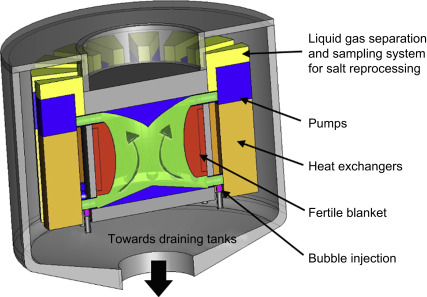
\includegraphics[width=.7\columnwidth]{msfr}
	\caption{Schematic diagram of the \gls{MSFR}. Retrieved from 
	\cite{allibert_7_2016}.}
	\label{fig:msfr}
\end{figure}

\subsection{Challenges in Multiphysics \gls{MSR} Modeling \& Simulation}

While modeling \glspl{MSR} is not necessarily more difficult than modeling
solid-fueled reactors, we must adapt our software tools to accurately model the
unique phenomena found in these circulating-fuel reactors. The differences in
the challenges of simulating \glspl{MSR} compared to solid-fueled reactors stem
mainly from the liquid fuel form of the fuel salt \cite{diamond_phenomena_2018,
huff_identifying_2019}.

Liquids generally exhibit greater thermal expansion per unit increase in temperature than solids.
The decreased fuel salt density due to thermal expansion
increases the likelihood of neutrons escaping the fuel region
and being absorbed by non-fissile material elsewhere in the reactor.
Consequently, combined with the temperature-dependent Doppler broadening of
resonance capture cross sections, \glspl{MSR} possess stronger negative fuel
temperature reactivity feedback than their solid-fueled counterparts
\cite{elsheikh_safety_2013}. These
phenomena ultimately result in strong interactions between the neutron fluxes
and the fuel salt temperatures, given that neutron fluxes affect fuel salt temperatures
through fission heat generation and fuel salt temperatures affect neutron
fluxes through the mechanisms described previously.

With the fuel salt also providing cooling in the core through advective heat
transfer, velocity flow
profiles in the fuel salts strongly impact the temperature distribution via
advection-dominated heat transfer \cite{diamond_phenomena_2018}. The flow-driven
temperature distribution contrasts
with the relatively static temperature profiles in fuel pins and
other solid fuel types, which are physically separate from the coolant.

\Glspl{DNP} flow freely within the primary coolant loop instead of
being held in place as in solid-fueled reactors. Thus, the delayed neutron
source distribution varies significantly depending on the flow profile and
velocity of the salt. In addition, the reactor loses some delayed neutrons from out-of-core
\gls{DNP} decay. These delayed neutrons are considered lost as they are emitted
in subcritical regions and are unlikely to contribute to further fission
reactions in the active core. The reduced delayed neutron fraction in the core
contributes to a greater prompt power spike following a reactivity insertion
event than solid-fueled reactors, absent any temperature reactivity
feedback.

Molten-salt flow along various parts of the coolant loop may fall within the turbulent flow
regime, characterized by chaotic eddies, vortices, and other flow instabilities.
Turbulent flow effects further complicate multiphysics interactions of flow with the temperature
and \gls{DNP} distribution. Turbulent flow effects contribute significantly to advection-dominated
heat and particle transfer in molten salt systems, thereby causing enhanced mixing. Therefore,
multiphysics software for \gls{MSR} analysis require adequate flow modeling capabilities with
support for \gls{DNP} drift and some form of turbulence modeling.

We require
\gls{MSR} simulation tools that possess transient modeling capabilities to simulate transient
accident scenarios. Furthermore, several transient scenarios involve control rods, either as active
safety mechanisms or as accident initiators through unintended control rod ejection. Therefore, we
also require \gls{MSR} simulation tools with accurate control rod modeling capabilities to run
numerical analyses of accident scenarios involving control rods.

\subsection{Moltres for Multiphysics \gls{MSR} Analysis}

Moltres \cite{lindsay_moltres_2017} is an open-source multiphysics reactor simulation software
explicitly developed considering \gls{MSR} characteristics in mind. Moltres is
built on the \gls{MOOSE} \cite{permann_moose_2020} open-source finite-element framework,
which facilitates multiphysics coupling between different
\gls{MOOSE}-based and \gls{MOOSE}-wrapped applications. The \gls{MOOSE} framework also provides
Moltres with advanced meshing and numerical solver capabilities through interfacing with libMesh
\cite{kirk_libmesh_2006} and PETSc \cite{satish_petsc_2019} open-source libraries. Therefore,
Moltres supports up to 3-D unstructured meshes, scales well on high-performance computing systems,
and provides a flexible multiphysics coupling system, which can be tailored for different types of
simulations.

Moltres models coupled neutronics and thermal-hydraulics in reactors. While
generally applicable to most reactor concepts, much of
Moltres' development focuses on meeting the needs of \gls{MSR} multiphysics simulations.
Together with \gls{MOOSE}'s \texttt{Heat}
\texttt{Conduction} and \texttt{Navier-Stokes} \cite{peterson_overview_2018}
modules, Moltres solves the multigroup neutron diffusion
equations for an arbitrary number of energy and precursor groups and
thermal-hydraulics equations simultaneously on the same mesh (or separately solved and coupled
through fixed-point iterations if desired).

Lindsay et al. \cite{lindsay_introduction_2018}
demonstrated Moltres' multiphysics \gls{MSR} modeling capabilities with 1-D salt
flow modeling in axisymmetric and 3-D models of the \gls{MSRE}. The neutron flux and
temperature distributions agreed qualitatively with legacy
\gls{MSRE} data albeit with some minor quantitative discrepancies due to
simplifications and assumptions in the reactor geometry. I demonstrated Moltres' capabilities for
1) looping of \gls{DNP} drift back into the reactor core, 2) coupling the \gls{DNP}
drift to numerically calculated salt flow profiles within the reactor core,
and 3) a decay heat model to simulate decay heat from fission products, with a 2-D axisymmetric
design of the \gls{MSFR} in my Master's thesis \cite{park_advancement_2020}.

While the Moltres
model of the \gls{MSFR} showed good agreement with other studies in most steady-state and transient
simulation cases, the Moltres model showed significant discrepancies during pump-initiated
transient scenarios without a proper turbulence model. Instead, the model applied a
uniform eddy viscosity assumption, which proved inadequate under non-steady flow. In order to
advance Moltres as a multiphysics simulation software for \gls{MSR} analysis, Moltres requires a
turbulence modeling capability to capture adequate turbulent flow phenomena and their interactions
with other physics present in \glspl{MSR}. Of the various classes of turbulence models, a
\gls{RANS}-based model is most suitable for coupling with Moltres when we consider computational
efficiency. The \gls{RANS}-based equations are time-averaged fluid flow equations
derived by separating the flow variable into its time-averaged and fluctuating components.
\gls{RANS}-based models are also well-validated, representing the most widely used turbulence
models for engineering applications.

In addition to new features, Moltres would benefit from further \gls{VV} of its existing
multiphysics capabilities to identify software bugs and ensure reliable results. Accurate modeling
and simulation of salt flow-induced \gls{DNP} drift and the strong coupling between neutronics and
thermal-hydraulics are crucial for \gls{MSR} simulation tools. Therefore, the
proposed work will include relevant \gls{VV} studies for Moltres.

\subsection{Control Rod Modeling in \glspl{MSR}}

Most reactor designs include control rods as a means to control the fission rate. Control rods
consist of strong
neutron absorbers like boron, cadmium, and gadolinium to absorb and thus reduce the number of
neutrons available to contribute to further fission chain reactions. All reactors start operation
with excess reactivity to ensure enough fissile material is available to last through to the next
scheduled refueling. Control rods and burnable poisons allow reactors to operate at a safe
multiplication factor by canceling out the excess reactivity. Control rods are also helpful
for ramping the power up or down during start-up, shut-down, or load-following operations. Most
importantly, control rods provide a safety mechanism for quickly shutting down a reactor under
dangerous conditions. Rapid control rod insertion is the primary mechanism of a reactor scram to
reliably introduce a large negative reactivity insertion in response to an unintended reactivity
insertion or other events that may threaten the reactor's safe operation. 

Amongst other tasks in reactor modeling, we aim to accurately reproduce control rod worth, which we
can measure as the relative reduction
in the neutron multiplication factor $k_{eff}$ due to the presence of the control rod in the
reactor. We are also interested in the accompanying change in flux shape near the
control rod. Neutrons entering the control rods are more likely to be absorbed than
adjacent regions in the reactor core. Therefore, control rods induce highly anisotropic neutron
angular fluxes and sharp gradients in the neutron flux in their vicinity. Control rods also cause
shifts in the neutron energy spectrum because their absorption cross sections are much higher in
the lower neutron energy range; more energetic neutrons generally have a higher probability of
escaping the control rod region. As a consequence, modeling control rods accurately requires
high-fidelity computational methods to capture the angular dependence in the neutron
flux near the highly absorbing medium. Existing reactor analysis workflows often rely on Monte
Carlo methods for high-fidelity neutron transport calculations.

However, neutron transport methods, like Monte Carlo, are very computationally expensive
and thus are mainly used for time-independent neutronic analyses. For solid-fueled reactors,
static control rod analyses can be justified due to the relatively static temperature distribution
shape in the fuel and disparate timescales of heat transfer from the fuel to
the coolant (seconds) and neutron flux changes (microseconds to milliseconds). In
\glspl{MSR}, this distinction blurs due to molten salt serving the dual role of fuel and
coolant and the strong fuel temperature reactivity feedback. For time-dependent multiphysics
simulations coupling neutronics to \gls{TH} and other physics present in nuclear reactors, most
reactor analyses rely on neutron diffusion theory for modeling neutronics. The issue with applying
neutron diffusion theory near control rods arises because neutron diffusion theory approximates
neutron transport theory by integrating over the angular variables. As a result, diffusion-based
methods perform poorly in reactor systems with control rods.

To tackle the issue of modeling control rods in \glspl{MSR} with the multigroup neutron diffusion
solver in Moltres, I will develop and implement a novel hybrid method for incorporating neutron
transport-derived corrections to the neutron diffusion method while largely preserving the
computational efficiency of the neutron diffusion method over neutron transport methods. This will
allow for computationally feasible transient analysis of \glspl{MSR} that incorporate thermal and
neutronic feedback on variable timescales.

\section{Objectives}

The overarching goal of this work is to improve on Moltres as a reliable, intermediate-fidelity
simulation tool for multiphysics \gls{MSR} analysis that can be run on workstations as well as on
larger computing clusters. Thus, new and existing capabilities in Moltres must
be accurate within accepted bounds, rigorously verified, computationally efficient, and highly
scalable. These conditions form the underlying development principles of the proposed work.

The scope of the proposed work can be divided into three main objectives. These objectives are:
%
\begin{enumerate}[itemindent=20pt, listparindent=1.5em, label=\textbf{\arabic*}]
  \item \textbf{verification and validation of existing multiphysics coupling capabilities in
    Moltres}

    Verify and validate existing multiphysics capabilities in Moltres for modeling and simulating
    the strong interactions between the neutronics and thermal-hydraulics in \glspl{MSR}. This
    objective will be met through two separate studies: verifying Moltres against the CNRS
    benchmark \cite{tiberga_results_2020} for fast-spectrum \gls{MSR} analysis, and modeling the
    \gls{MSRE} zero-power pump start-up and coast-down experiments. I will perform the second study
    in collaboration with the developer of QuasiMolto \cite{reynolds_analysis_2023} as a \gls{VV}
    study with the additional aim of creating a reproducible numerical benchmark of the listed
    \gls{MSRE} experiments.

  \item \textbf{implementation of a \gls{RANS}-based turbulence model in Moltres, and}

    Implement a Spalart-Allmaras turbulence model in Moltres to support turbulent flow simulations
    in \gls{MSR} analyses. This objective addresses the absence of turbulence modeling capability
    in Moltres and the consequent restriction on Moltres for modeling \gls{MSR} systems with
    complex turbulent flow.

  \item \textbf{development of a novel hybrid method to improve control rod modeling in Moltres}

    Develop a novel hybrid $S_N$-diffusion method for improved modeling of \gls{MSR} systems with
    control rods. The hybrid method uses the discrete ordinates ($S_N$) method for solving the
    neutron transport equations to generate corrections for the diffusion-approximated streaming
    term in the neutron diffusion equations. The $S_N$ calculations are high-level
    calculations on a reduced problem domain containing the control rods to minimize computational
    expense.
\end{enumerate}

\section{Outline}

Chapter 2 presents a literature review of existing multiphysics \gls{MSR} simulation software,
\gls{VV} studies on \gls{MSR} modeling and simulation, turbulence modeling in \gls{MSR} systems,
and correction techniques for neutron diffusion methods.
Chapter 3 describes Moltres and its existing capabilities in the context of previously published
work.
Chapter 4 summarizes the findings of the first verification study under the first objective: the
verification of Moltres for multiphysics \gls{MSR} modeling against the CNRS benchmark.
Chapter 5 presents the theory and preliminary results of the novel hybrid $S_N$-diffusion
method for the third objective.
Chapter 6 details the proposed work to fully meet the three objectives.
